%VETB Report
\documentclass{report}
\author{Tym Pakulski - University of Bath}
\title{Internal Volume Measurement Device}
\date{September 2013 - August 2014}

\usepackage{graphicx}
\usepackage{amsmath}
\setlength{\parindent}{0pt}
\begin{document}
\graphicspath{{./images/}}
\maketitle
\tableofcontents
\section{Introduction}
Leak testing of the CMS various cooling systems is a regular exercise that currently relies on a 'rule of thumb' approach to test specifications. True allowable leak rates are defined in terms of a percent of total internal volume per unit time, but exact numbers for the internal volumes of the various subsystems are difficult to establish. A device that can measure the internal volume of existing systems would be useful to quantify allowable leak rates and streamline the leak testing process.
This report documents the proof-of-concept phase of a rig that will be used to measure internal volumes by injecting them with gas and measuring the rate of pressure change. 
\subsection{Theory}
The volume measurement concept comes from the ideal gas law \eqref{ideal}, and the equation for molar volume \eqref{molarVolume}. It assumes constant temperature and volume. All units are S.I.

\begin{eqnarray}
PV = nRT \label{ideal}\\
V_{mol} = \frac{RT}{P} \label{molarVolume}\\
n = \frac{PV}{RT} \nonumber \\
\frac{dn}{dt} =  \frac {V}{RT} \frac {dP}{dt} \nonumber \\
\frac{dV_{in}}{dt} =  \frac{RT}{P} \frac {V}{RT} \frac {dP}{dt} \nonumber \\
V = \dot{V_{in}} dt \frac{P_1}{P_2 - P_1}
\end{eqnarray}
An alternative derivation supplied by Roberto Guida assumes standard conditions to calculate the molar volume. While slightly more complex, this formulation has the advantage of taking flow controller readings directly as input, as it corrects for ambient temperature different from the flow controller calibration. See \ref{sec:operatingPrinciples}.
\begin{eqnarray}
PV = nRT \nonumber\\
V_{mol} = 22.4 \text{ [L]}\\
n = \frac{PV}{RT} \nonumber \\
\frac{dn}{dt} =  \frac {V}{RT} \frac {dP}{dt} \nonumber \\
\frac{dV_{in}}{dt} =  \frac{22.4}{R} \frac {V}{T} \frac {dP}{dt} \nonumber \\
\dot{V}_{in}\text{ [l]} = 2.69\frac{V}{T} \frac{P_2 - P_1}{dt} \nonumber \\
V = \frac{\dot{v}_{in}}{2.69} \frac{T}{P_2 - P_1}\nonumber \\
V\text{ [cm$^3$]} = \frac{\dot{v}_{in}\text{ [l/hour]}}{3600}\frac{dt\text{ [s]}}{P_2-P_1 \text{ [bar]}}\frac{T\text{ [$\,^{\circ}\mathrm{C}$]}+273}{269}1000 \label{roberto}
\end{eqnarray}
\begin{figure}[h]\label{schematic}
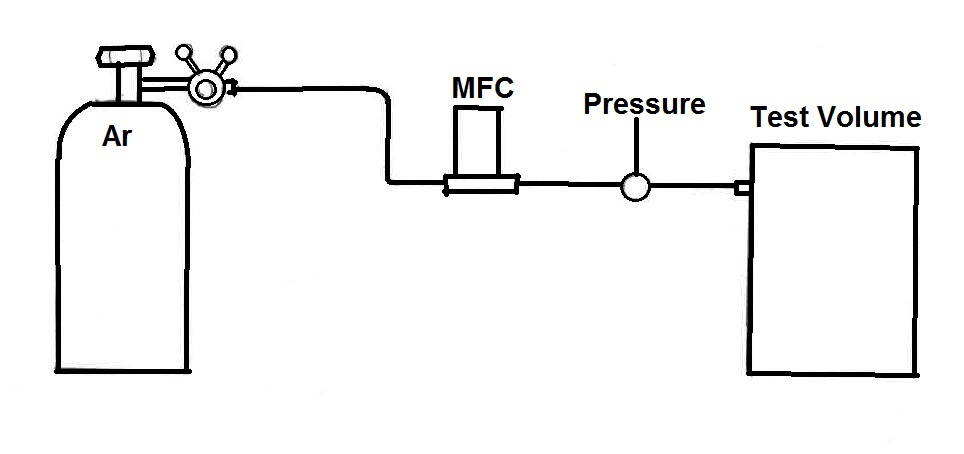
\includegraphics[width=\textwidth]{schematic}
\caption{Schematic of the volume estimation concept}
\end{figure}
\\
\subsection{Specifications}
The volume estimation product should be:

\begin{itemize}
	\item{Compact and transportable}
	\item{Simply designed and accessible for untrained users}
	\item{Sufficiently accurate to meet the leak test specification accuracy}
	\item{Usable without a laptop or expensive data logging equipment}
	\item{Low-power}
\end{itemize}

\subsubsection{Accuracy Specification}
The accuracy of the device is constrained by the allowable errors in the devices uses. An error in the calculated volume will affect the accuracy of both the \textit{allowable} leak rate and the \textit{measured leak rate}. See appendix %\ref{LEAKS}S
	
\subsection{State of the Project}
So far, the volume estimation concept has been tested using a pressure transmitter and DAQ of Norbert Frank's pressure decay measurement rig in building 27, shown in Figure \ref{b27}. Two different flow meters have been used to measure the volume of a dive bottle. 
\begin{figure}[h] \label{b27}
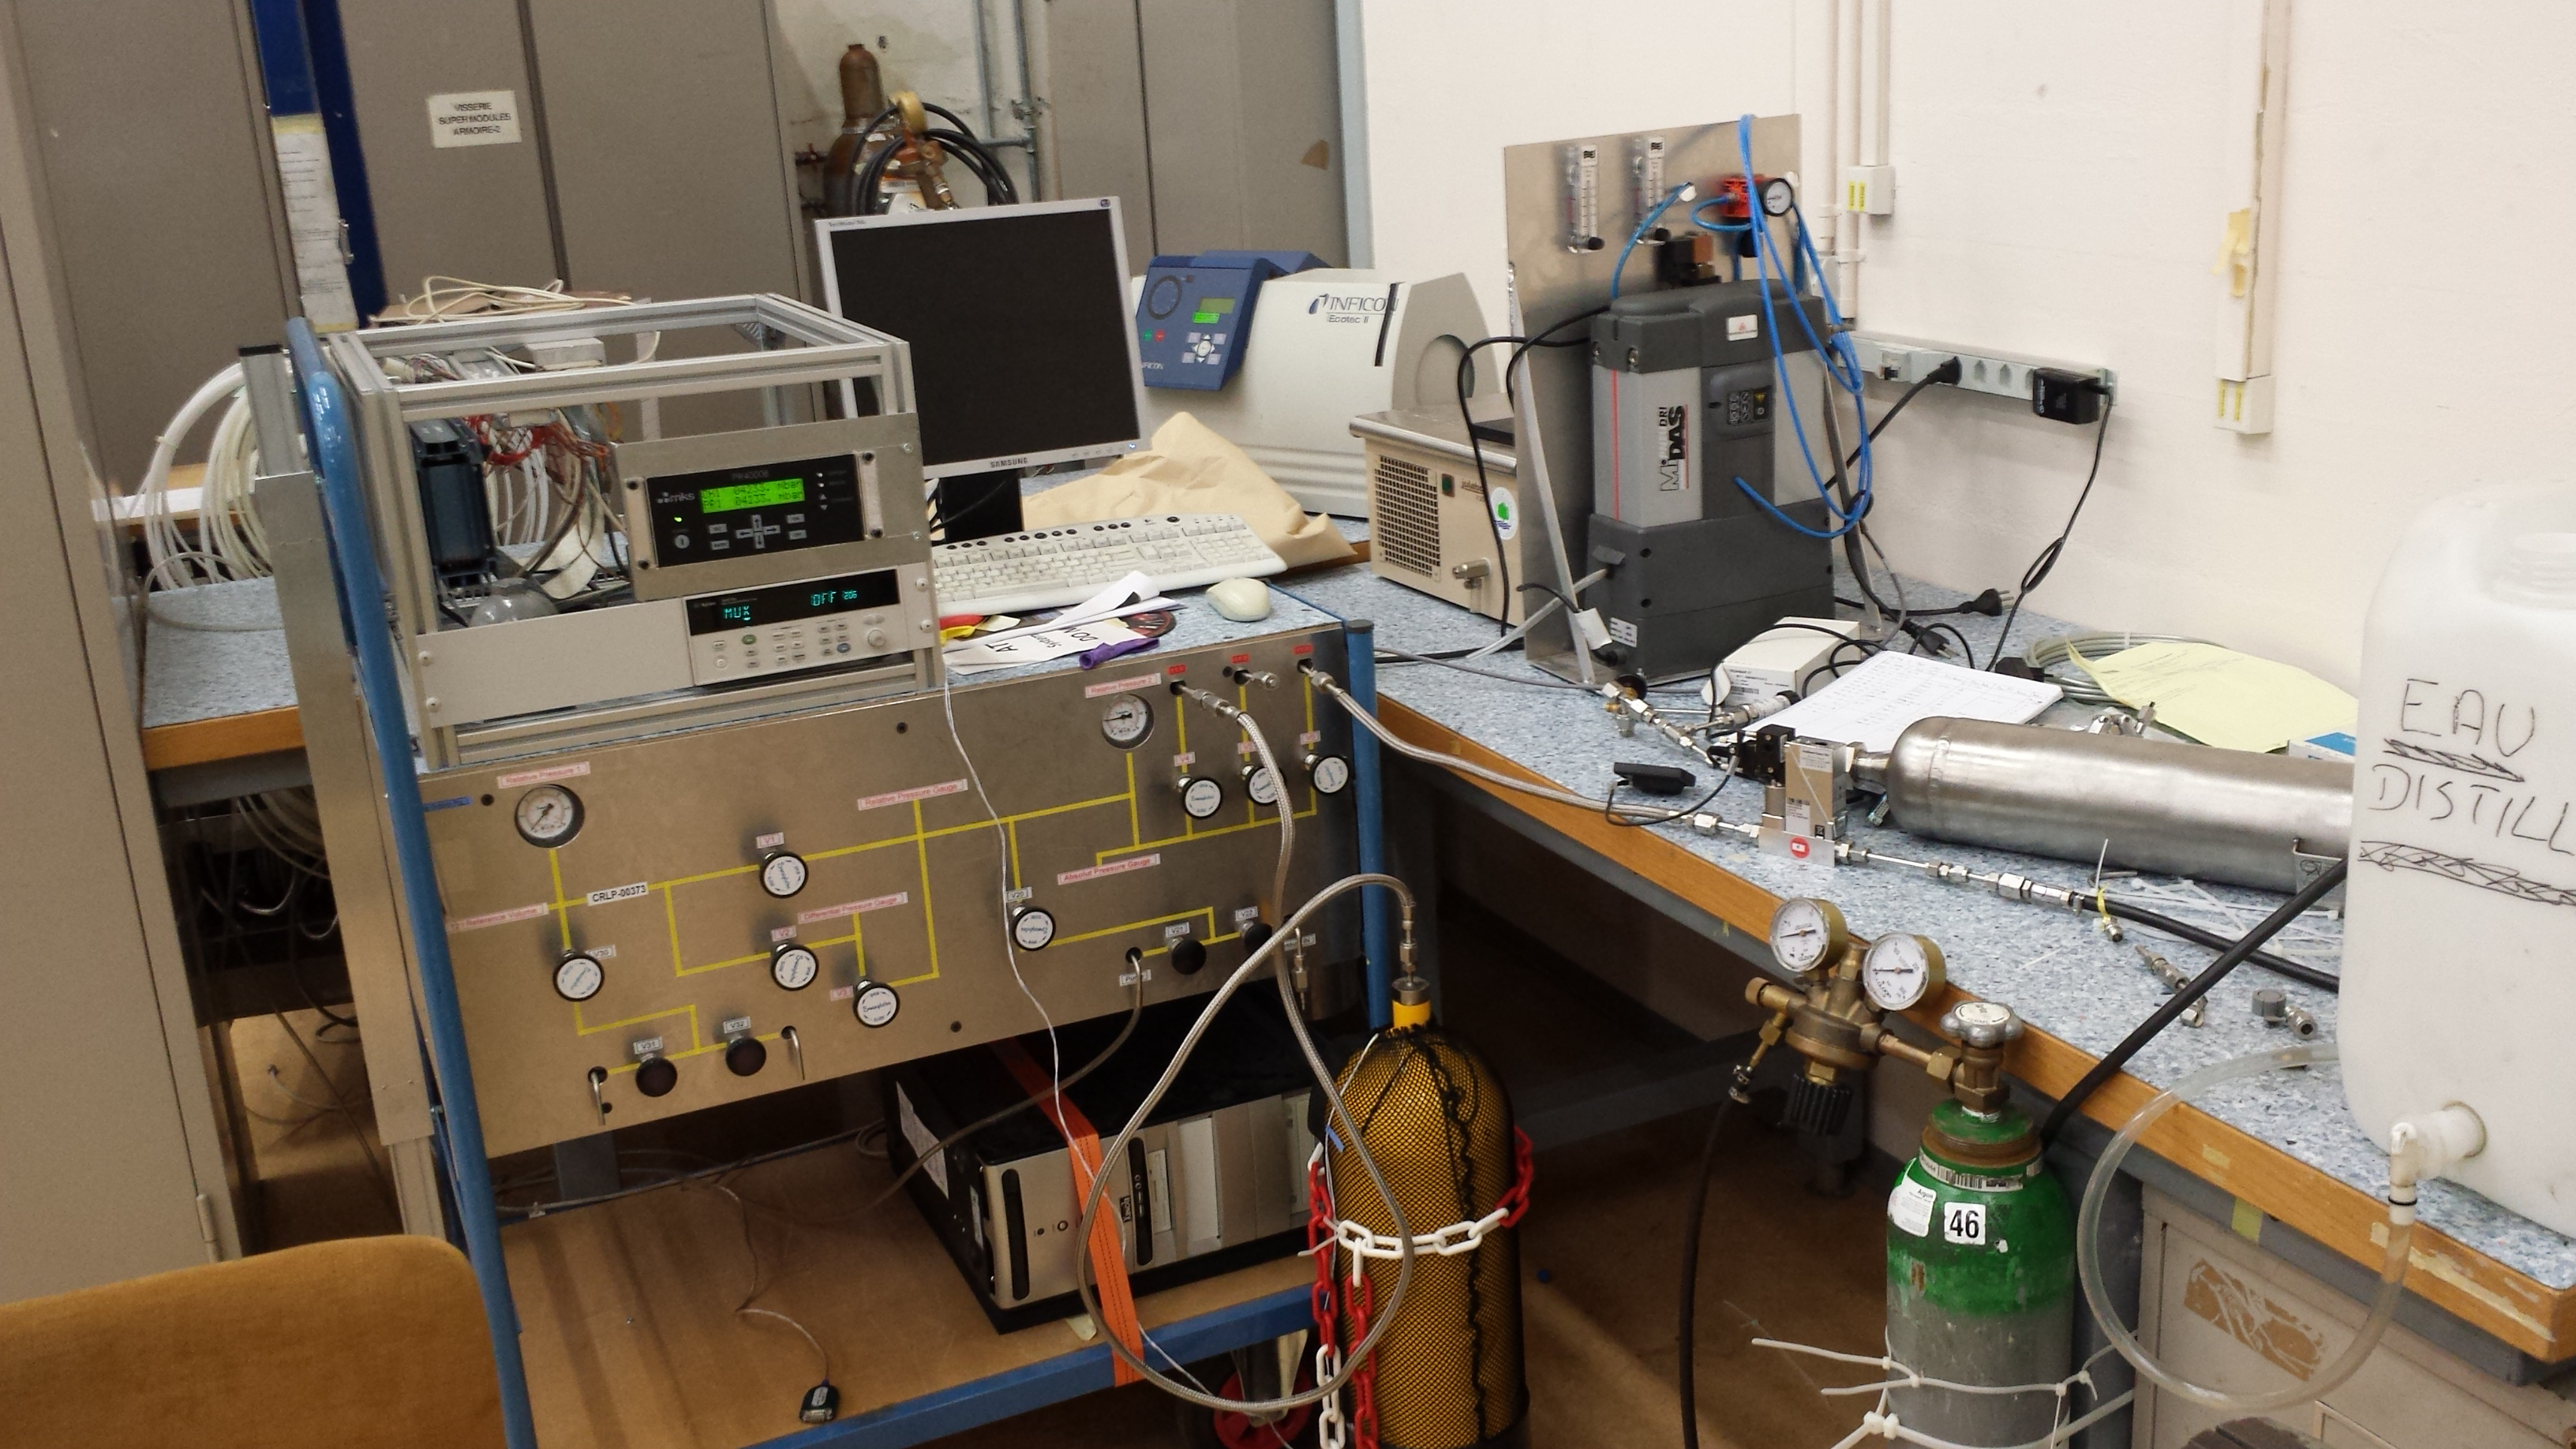
\includegraphics[width = \textwidth]{wide}
\caption{The test rig in building 27.}
\end{figure}
\subsubsection{Using the Building 27 Rig}
DAQ is handled by a labVIEW module on the local PC. The .vi, saved to the desktop, is called \textit{MAIN\textunderscore ScanChannels.vi}. Tests can be run from the \textit{Stand1} tab on the front panel. The data for each test is saved to a .txt file in a folder at \textit{C:/Project/PressureTest/Data/}. The useful channels are the time and the first pressure signal: \textit{absSysPressure}. The PC also has installed Bronkhorst's Flow DDE and Flow Plot software, which can be used to change the MFC set point and log its 3 channels through RS232. \\
The rig is connected to the 15 L (true volume) dive bottle with 1/4" VCR fittings. The bottle's volume was confirmed by filling it with water and measuring its change in weight. \\
The rigs gas inlet, purge line and fluid connection are controlled by valves shown in Figure \ref{valves}.
\subsubsection{Relevant Contacts}
\begin{itemize}
	\item{Norbert Frank: 16 }
	\item{Patrick Carrier: }
	\item{Tym Pakulski: tsp26@bath.ac.uk}
\end{itemize}


\begin{figure}[h] \label{valves}
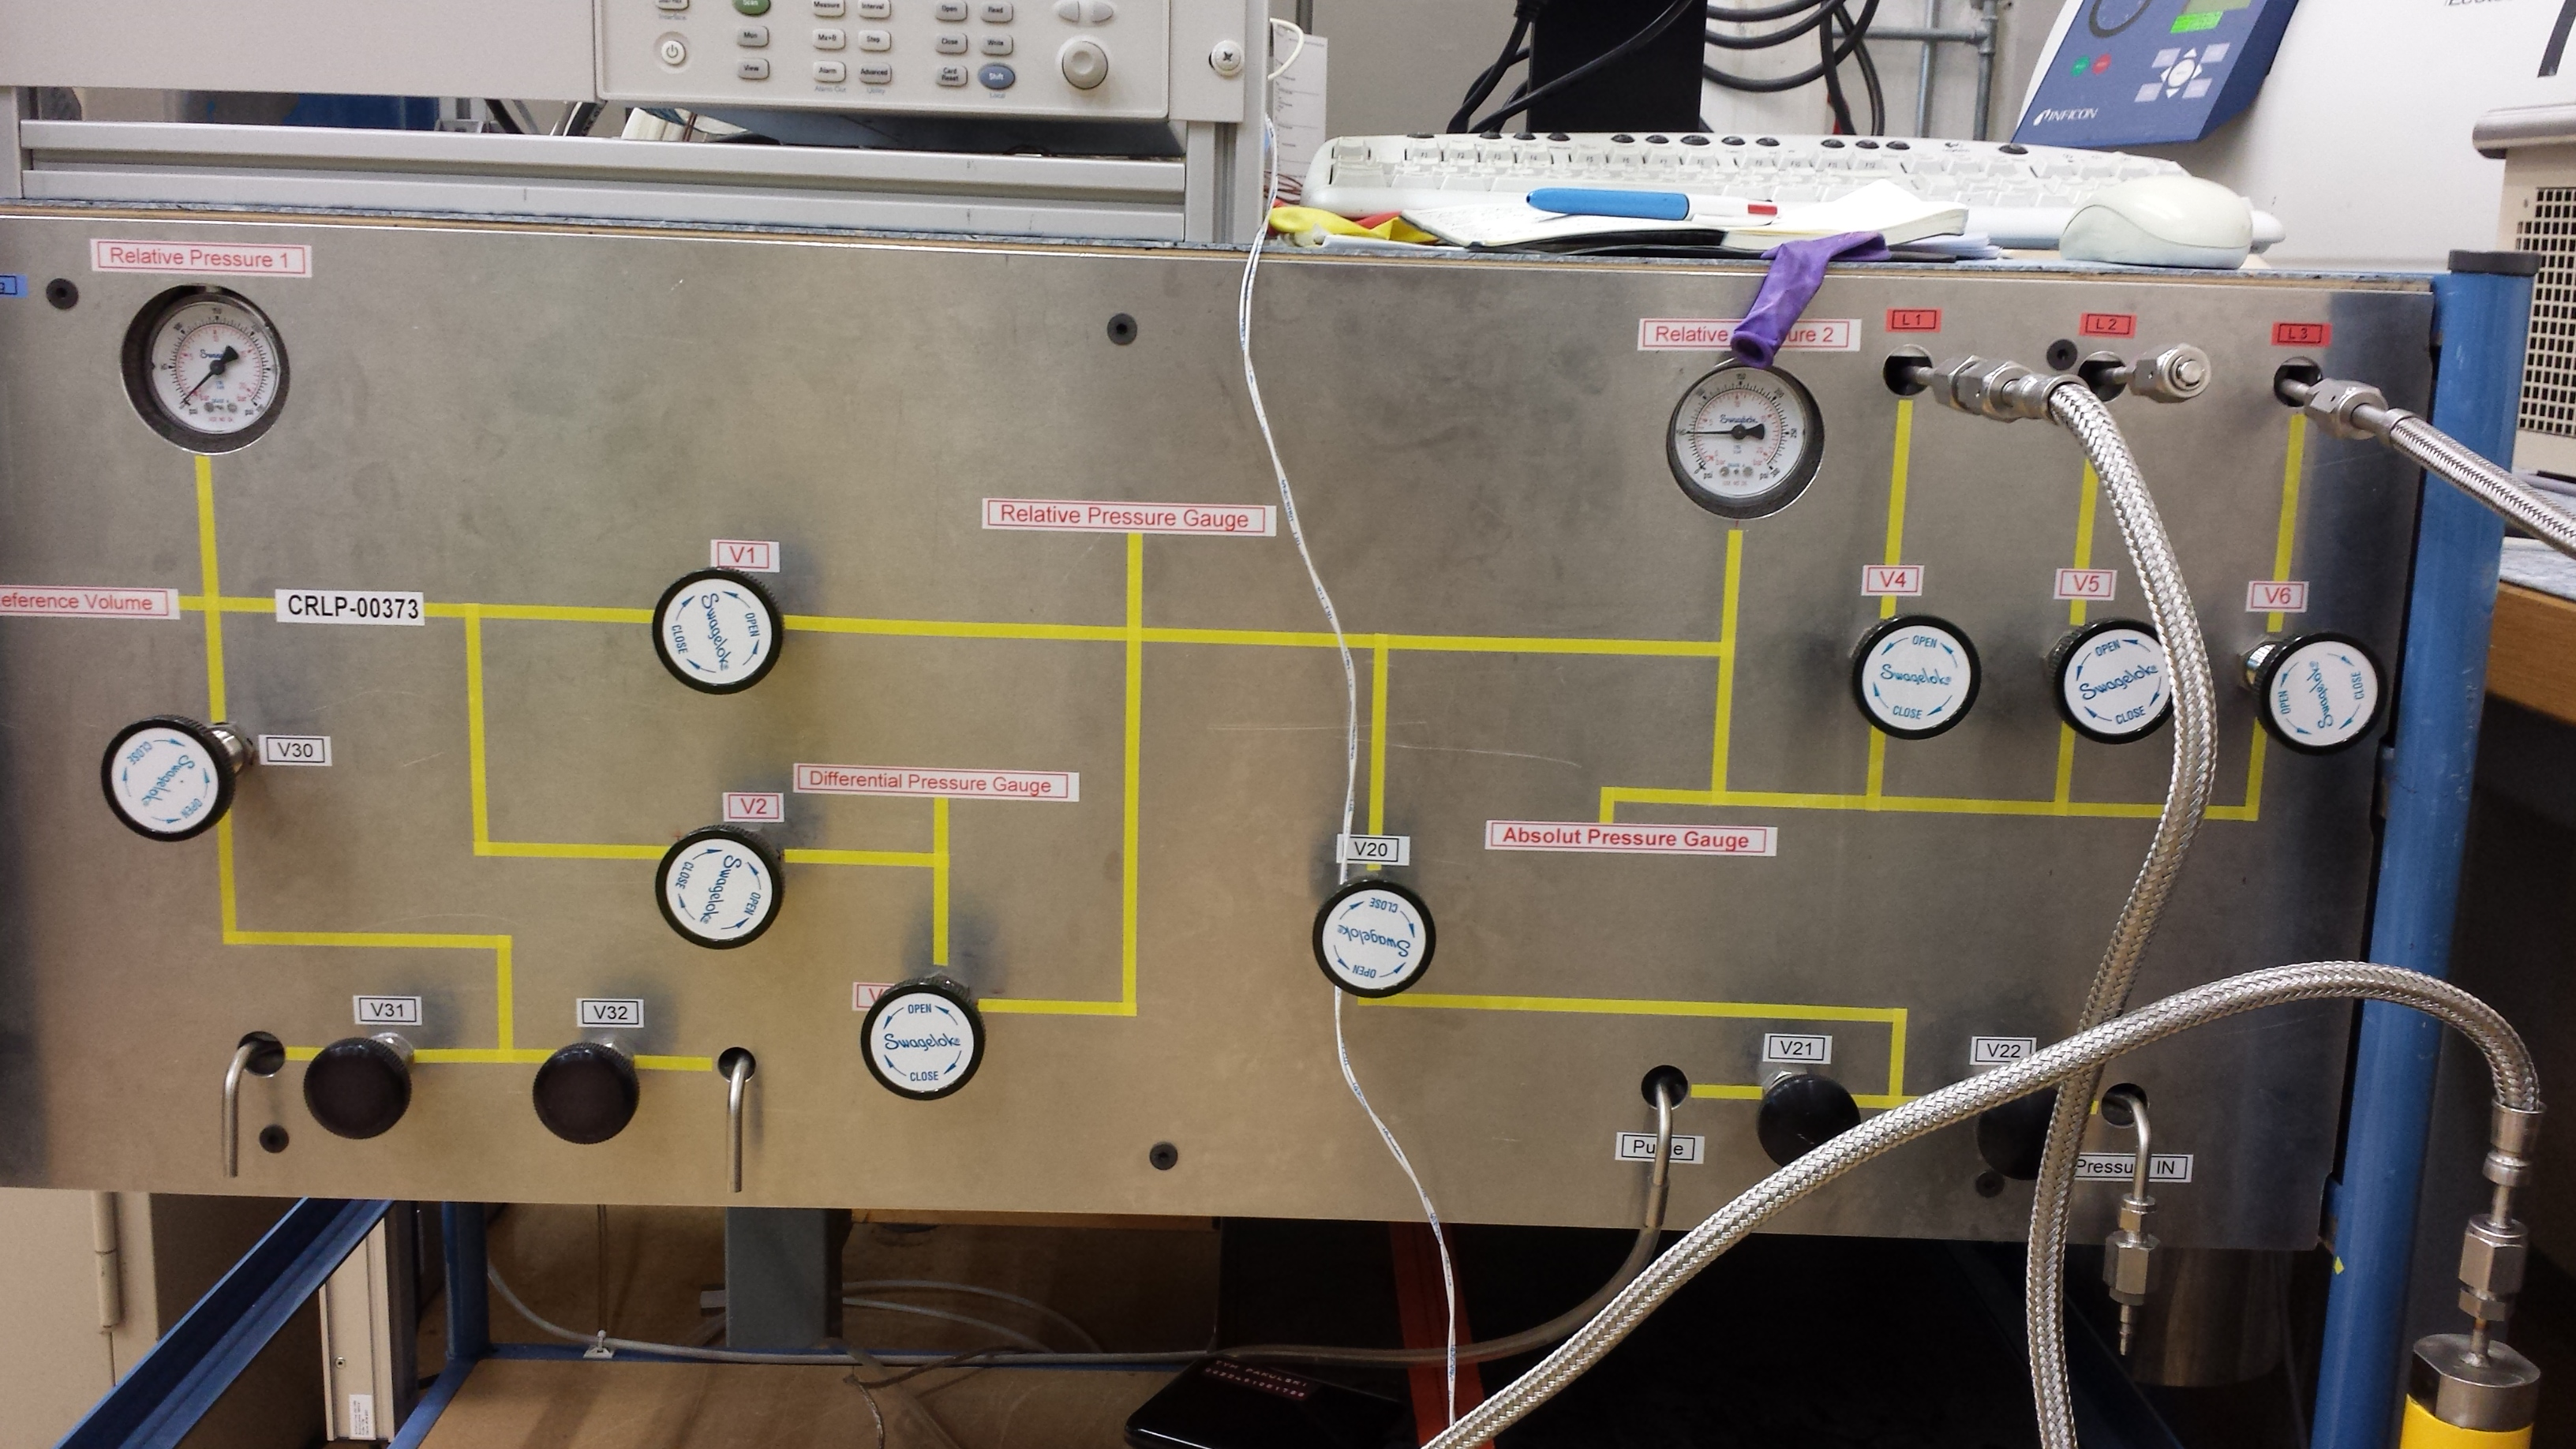
\includegraphics[width=\textwidth]{valves}
\caption{V6: fluid inlet, V4: Test volume, V20 and V21: Purge, V1 and V3: keep closed}
\end{figure}

Valve 4 connects to an unused part of the rig and is kept close to minimise pipe volume.

\section{Instrumentation and DAQ}
\subsection{Bronkhorst Flow Controllers}
The first iterations of the rig have used Bronkhorst flow controllers of type  and . These were borrowed from Patrick Carier in the gas group 16.. 
\subsubsection{Operating Principles} \label{sec:operatingPrinciples}
The controllers operate on the thermal mass flow principle, and measure the mass of fluid passing through their regulation valve as a function of the power needed to heat a temperature probe a set distance away in the flow. See appendix. The instruments take a $L_n$ per minute set point via RS232 bus, which they convert for their grams per second control logic using equation \eqref{molarVolume}. In other words, the instruments are calibrated for a specific fluid, inlet pressure and fluid temperature. \textbf{It is essential that these parameters are respected.}
\\
In practice, this means using the correct fluid and adjusting the downstream pressure of the reducer to match the value specified in the controller firmware and typically marked on the side of the device. Ambient temperature is more difficult to adjust. Instead, it is good practice to check the calibration temperature, which is typically 273 K, and multiply the volumetric flow rate by a 'temperature gain', as shown in \eqref{temperatureGain}
\begin{equation} \label{temperatureGain}
\dot{V}_{true} = \dot{V}_{set point}\frac{T_{true}[K]}{T_{calibrated}[K]}
\end{equation}
\\
Alternatively, the temperature gain can be applied to the calculated volume itself. If the derivation supplied by Roberto Guida is used, the temperature difference can be ignored. \\

\section{Problems with Flow Controllers}
Two major problems were encountered during early iterations of the project. 
The first version of the instrumentation seemed to exhibit random errors in calculated volume in the order of 10, well beyond those predicted by theory. Second, a unexpected correlation between injection flow set point and calculated volume was observed. 
Both problems were resolved by a change of flow controller. \\
It appears the most likely explanation for the systematic error is a leak in the instrumentation section. In general, a faster flow rate means a larger integral of pressure with respect to time, which causes a higher net leak flow out of the system. Thus the higher the flow rate, the greater the error due to leaks. 
No leaks were found in several sniffer tests conducted with both $CO_2$ and helium. However, pressure drops in the instrumentation section  consistent with a leak were observed.
The random error in calculated volume was most likely due to temperature variations. Minor temperature variations first appeared trivial. While the temperature term is eliminated in the first formulation of the derivation used for data analysis, it can be expressed as a pressure error using the ideal gas law. The linear error implies that the typical 3 degree temperature fluctuations observed were insignificant. \\However, the derivation itself rests on the assumption of constant temperature, and the 1 percent error is enough to invalidate the concept. \\
The new controller, with 10 times the maximum flow of the old one,  eliminated the systematic error with leak tight connections, and  led to fast-flow tests too short for significant temperature fluctuations. While the old controller required 8-14 hour tests for the 15 L volume, the new one could achieve 1 bar of dP in 30 minutes.
\subsection{DAQ}
Estimating volume requires, at a minimum, two data points of time and pressure and the flow set point. A temperature reading is useful to eliminate a minor systematic error if temperature is constant, or to detect a change in temperature that would void the test. More time and pressure data reduce random errors. \\
The current rig measure pressure through a 4-20 mA current loop connected to a LabVIEW module. The software can log pressure and time in this way. Future iterations of the project will probably simplify the DAQ process by saving the current loop readings with time stamps to a USB storage device. This will allow the test to be run without a laptop. 
\section{Analysis tools}
%ALTERNATIVE FORMULATION: SLOPE INTERPRETATION
%WHERE TO FIND MATLAB ETC
%PYTHON SCRIPTS
\section{Recommendations}
The next iteration of the product should evaluate its accuracy for smaller test volumes of 2-3 litres. If the system's performance meets accuracy specifications, focus can shift to selecting permanent components with the correct parameters.

Future iterations should respect the following findings about the instrumentation
\begin{itemize}
	\item The inlet pressure on the flow meter must match the calibration pressure  in the firmware.
	\item The test volume temperature must be kept constant.
	\item Tests should be kept short to minimise temperature variation. 
	\item A temperature gain should be applied to the calculated volume if rig temperature differs from the calibrated temperature.
	\item A fast flow meter in the order of 1 l/min appears to offer a good balance of short test duration and flexibility for test volumes of interest.
	\item The rig must be leak tight.
\end{itemize}	
With instrumentation ordered, final design development should focus on the user experience, specifically the software. With 4-20 mA current readings saved to the USB drive, a simple program should be written to fetch the data 
Once a minimum viable product has been established, two further developments are worth investigating:
\subsubsection{Monitoring temperature} 
A temperature measurement is useful to be able to quantify the temperature gain that should be applied to the volume calculation to account for the difference in gas temperature and calibration temperature. Further, a running temperature measurement can be used to check whether significant temperature changes occur during the test, which would void the data.\\
The former could be achieved with something as simple as an analogue thermometer somewhere on the rig, assuming a constant temperature throughout the test. The latter would require dedicated hardware and DAQ to store the signals, which would likely be incompatible with the 4-20 mA pressure signals. With short tests, it can be argued that it is safe to assume constant temperature throughout the test.
\subsubsection{Pressure decay test capability}
The rig could also be used for pressure decay testing. By adding a valve upstream of the pressure sensor as shown in Figure \ref{schematicWithValve}, the pressurised test volume can be sealed, and the pressure transducer can be used to record pressure drop over time. 
\begin{figure}[h]
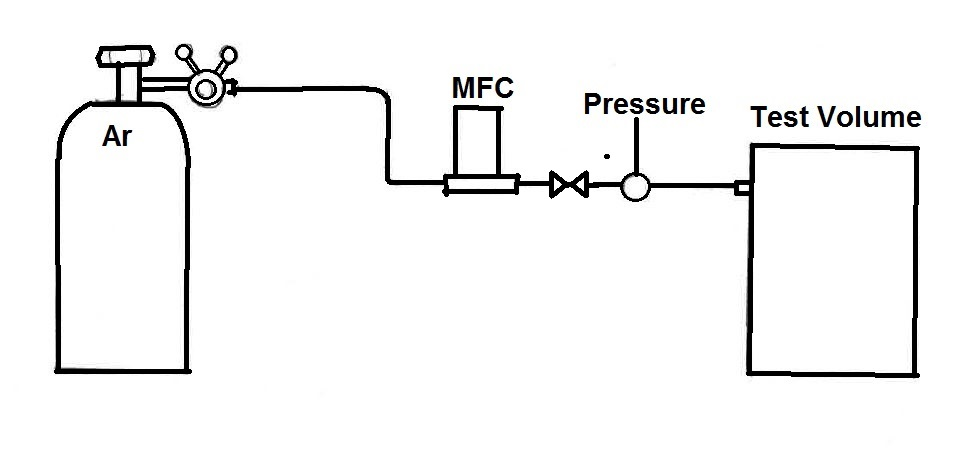
\includegraphics[width=\textwidth]{schematicWithValve}
\caption{The volume estimation instrumentation with an added valve for pressure decay testing.}
\label{schematicWithValve}
\end{figure}
This would could prove particularly convenient in the CMS, as it would allow both the volume estimation and the pressure decay test without purging the system or disconnecting the fittings. The device would first be connected to the pressure reducer and the test volume. Argon would be injected and pressure measured to calculate the volume. Then, the valve would be closed and pressure drop measured. With the pressure drop, the time, and the calculated volume, the leak rate can be calculated. 
\end{document}


